\documentclass[tikz]{standalone}
\usepackage{tikz}
\usetikzlibrary{positioning, graphs}
\usetikzlibrary{graphs.standard}
\begin{document}
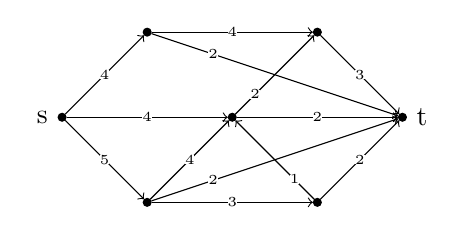
\begin{tikzpicture}
	[vertex/.style={draw,circle,inner sep = 0mm, minimum size = 1mm, fill = black},
	 edgelabel/.style = {fill = white, inner sep = 0mm, font=\tiny}]
	\node[vertex, label = left : s] (s) at (0,0) {};
	\node[vertex] [above right = of s] (a) {};
	\node[vertex] [below right = of s] (b) {};
	\node[vertex] [below right = of a] (c) {};
	\node[vertex] [above right = of c] (d) {};
	\node[vertex] [below right = of c] (e) {};
	\node[vertex, label = right : t] [above right = of e] (t) {};
	
	\draw[->] (s) to node[edgelabel] {$4$} (a);
	\draw[->] (s) to node[edgelabel] {$5$} (b);
	\draw[->] (s) to node[edgelabel] {$4$} (c);
	\draw[->] (a) to node[edgelabel] {$4$} (d);
	\draw[->] (a) to node[edgelabel, near start] {$2$} (t);
	\draw[->] (b) to node[edgelabel] {$4$} (c);
	\draw[->] (b) to node[edgelabel] {$3$} (e);
	\draw[->] (b) to node[edgelabel, near start] {$2$} (t);
	\draw[->] (c) to node[edgelabel, near start] {$2$} (d);
	\draw[->] (c) to node[edgelabel] {$2$} (t);
	\draw[->] (d) to node[edgelabel] {$3$} (t);
	\draw[->] (e) to node[edgelabel, near start] {$1$} (c);
	\draw[->] (e) to node[edgelabel] {$2$} (t);
\end{tikzpicture}
\end{document}